\chapter{Background on Human Activity Recognition using Wearable sensors} \label{chap:background}
\section{Background }
In this section, we provide an overview of a typical activity recognition process, aka ARP, explain and compare different sliding windows techniques and describe common evaluation methods in HAR.
\subsection{Activity Recognition Process}\label{subsec:ARP}

\begin{figure}[ht]
    \centering
    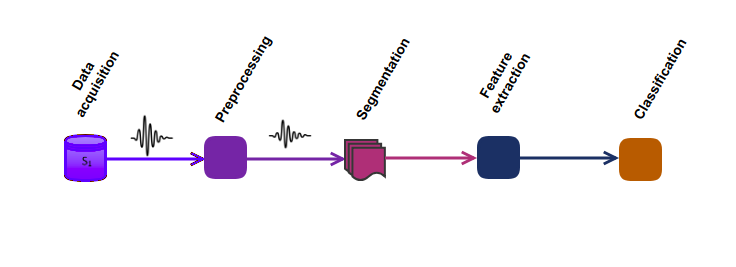
\includegraphics[width=1\textwidth]{Figures/HARP.png}
    \caption{Human activity recognition process}
    \label{fig:tsprocess}
\end{figure}

ARP is composed of a sequence of signal processing, pattern recognition, and 
machine learning techniques~\cite{bulling2014tutorial}. It mainly 
consists of 5 steps, shown in Figure \ref{fig:tsprocess} and 
explained hereafter.

\begin{figure}[ht]
    \centering
    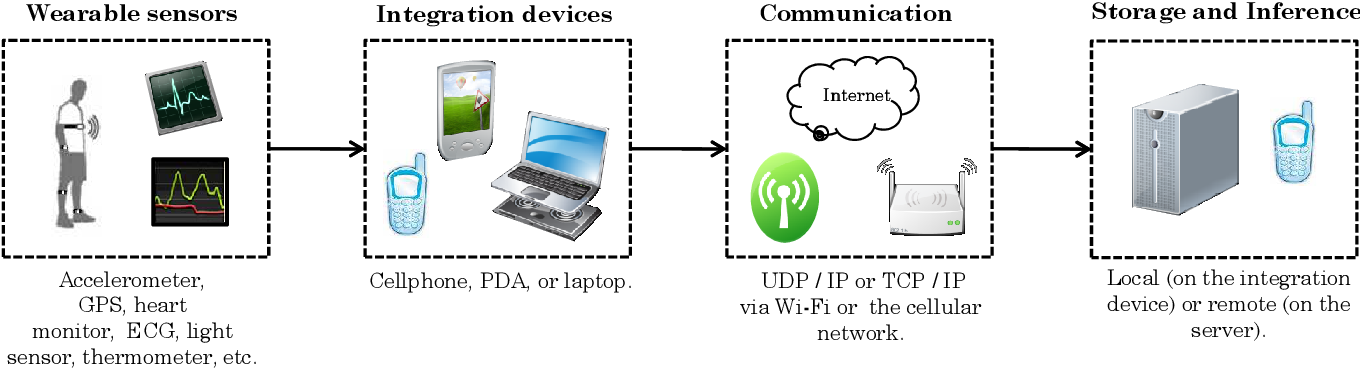
\includegraphics[width=.9\textwidth]{Figures/general_data_acqu.png}
    \caption{Generic data acquisition architecture for HAR extracted from~\cite{lara2012survey}}
    \label{fig:data_aqc}
\end{figure}

\subsubsection{Data acquisition} Several sensors are attached to different body parts. They mostly acquire 3D acceleration, gyroscopic and magnetic field measurements, etc, which measure different attributes such as  motion~\citep{iglesias2011ubiquitous}, location~\citep{choujaa2008tracme}, temperature~\citep{parkka2006activity}, and ECG~\citep{jatoba2008context}. Sensors discretize signals at a given frequency, typically 50Hz for 
daily activities or 200Hz for fast sports, and transmit data through UDP/IP or TCP/IP protocols to integration devices (ID) to be preprocessed~\citep{lara2012survey}. IDs can be different devices including cellphones, PDAs, laptops or a customized embedded systems~\citep{lara2012survey}. Figure~\ref{fig:data_aqc} shows a generic architecture of data acquisition in HAR. It should be noted that all of the mentioned components are not necessarily implemented in every HAR systems.      
 

\subsubsection{Preprocessing} Data points coming from sensors may
include artifacts of various origins such as 
electronic fluctuations, sensor malfunctions, and physical activities~\cite{bulling2014tutorial}. To eliminate such artifacts, filtering techniques are commonly applied, such as the Butterworth low-pass filter, which flats the coming signals as much as possible through rolling off down the higher frequencies beyond the cut-off point to zero ~\cite{morris2014recofit,selles2005automated,najafi2003ambulatory}. In any case, preprocessing techniques need to preserve
the signal characteristics that carry relevant information about the activities and consequently, they should be used with care as they may remove valuable information from the signals.


\subsubsection{Segmentation}
In this stage, the coming signals from sensors are partitioned into time windows labeled from the most frequent activity in the window. There are several ways to segment the sensor signals in HAR field which can be categorized into three groups, namely activity-defined windows, event-defined windows and sliding windows~\cite{banos2014window}. 

\noindent\textbf{Activity-defined windows}- In this technique, signals are partitioned based on the detection of activity changes, so the start and end points of each activity should be determined. Since the times of activities can be different, the window sizes are not fixed. In the literature, several methods have been used to identify the activity-transition points. For instance,~\citep{sekine2000classification,nyan2006classification} suggest a model based on the variations in the frequency characteristics to identify activity-transition points.  Another example is work in~\citep{yoshizawa2013parameter} which propose a heuristic method to separate static actions from dynamic ones. In the simpler scenario, the activity-transition points can be identified by user feedback~\citep{lester2006practical,he2009activity,figo2010preprocessing,dernbach2012simple}. 

\noindent\textbf{Event-defined windows}- Some activities such as meal preparation could be better recognized as a sequence of actions performed in a certain order. However, such activities are irregular and the order of actions for a specific one can be different and under such circumstances, the identification of specific events is particularly advised. The goal of event-defined windows is locating specific events in the signals to be used for data segmentation. In particular, this method is widely used in Gait analysis~\citep{banos2014window}. In this case, the models aim to detect heel strikes (the initial floor contact) and toe-offs (the end of floor contact) events. In the literature, several methods have been utilized to identify such events including analyzing the foot's linear acceleration~\citep{aminian1999temporal,selles2005automated}, Foot~\citep{aminian2002spatio} and shank~\citep{jasiewicz2006gait} sagittal angular velocity, using clustering models such as Gaussian mixture~\citep{aung2013automated}, using external mechanisms like stopwatch to register the first crossing time of hind foot and lead foot from a given start and end lines respectively~\citep{dobkin2011reliability}, etc. Identifying such events, subsequently can be used to recognize activities. For example,~\citep{benocci2010wearable} uses a model to recognize walking by identifying the gait cycle on a single foot tagged through a heel strike event. Like activity-defined windows, the window sizes are not fixed since the events may not be uniformly distributed in time.  

\begin{figure}[htp]
  \centering
  \subfigure[Non-overlapping]{
\label{subfig:NOSW}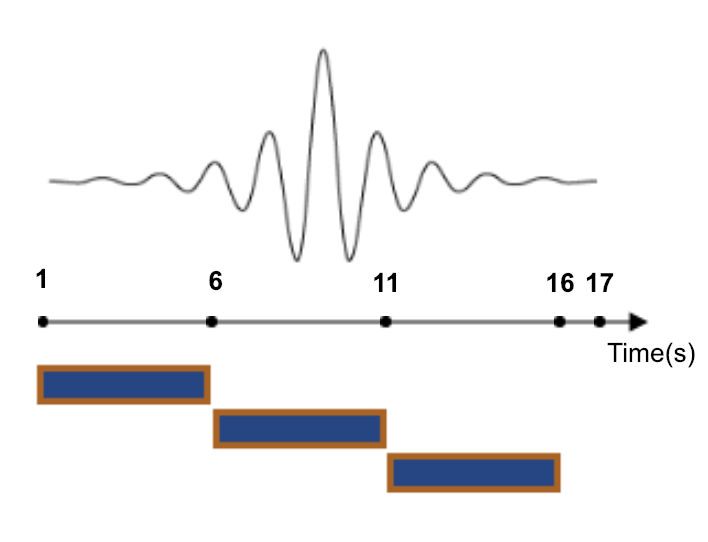
\includegraphics[scale=0.5]{Figures/NOSW.png}}\quad
  \subfigure[Overlapping-2 s sharing ]{\label{subfig:OSW}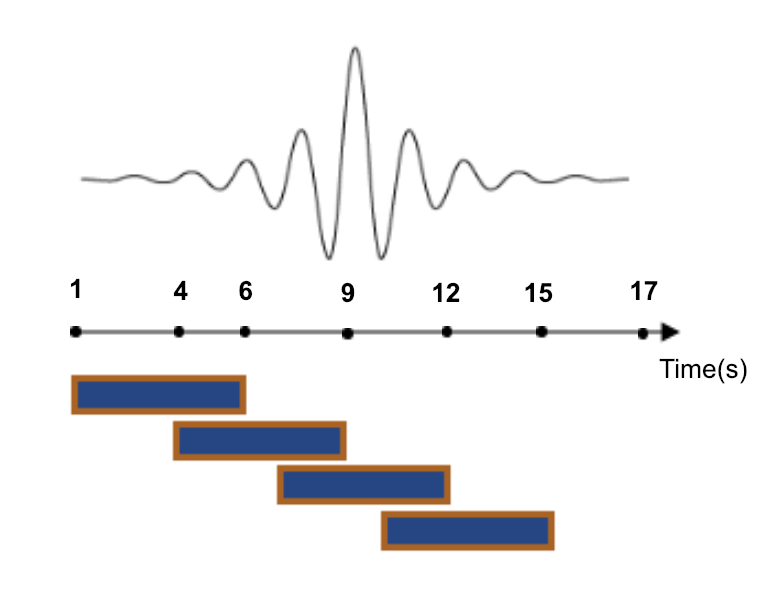
\includegraphics[scale=0.5]{Figures/OSW.png}}

   \caption{5-second sliding windows. }
   \label{fig:SlidingWindow}
\end{figure}

\noindent\textbf{Sliding windows-} The sliding window approach is the most widely used method in the segmentation step of ARP due to its implementational simplicity and lack of preprocessing~\citep{banos2014window}. In this approach, the sensor signals are split into windows of fixed size. If there is overlap between adjacent windows, this technique is known as overlapping sliding window, and if not, it is called non-overlapping windows technique. 
Figure~\ref{fig:SlidingWindow} illustrates the 
non-overlapping and overlapping windowing techniques.

\noindent\textbf{Formal definition-}
Mathematically, a sliding window process can be defined as follows.
Assume a stream of data values $x_i \in \mathbb{R} $ at times $t_i(i \in \mathbb{N})$. For simplicity, we assume that $t_0 = 0$ and the sampling period remains constant at $\Delta{T}$, i.e., 

$\forall i \in \mathbb{N}, t_{i + 1} - t_i = \Delta{T}$.

A fixed length sliding window splits the data stream into individual segments, where each segment
consists of n $(n \in \mathbb{N},n>1)$ samples. Consequently, the window size T in seconds is computed as follows:

$T = (n-1)\Delta{T}$,

where $\Delta{T}$ is the sampling period. We also denote $p \in {\{0,1,2,...,n-1\}}$ as the number of samples that are
within the overlapping period between two consecutive windows, where p = 0 refers to the
scenario with non-overlapping windows. Next, the overlapping period between two consecutive
windows in seconds, i.e., OP, can be computed as follows:

$OP = p\Delta{T}$.

Many research articles define the overlapping period as a percentage of the overall window length,
e.g., 80\% overlapping windows. The overlapping period in percentage can also be found as follows:

$ OP(\%) = \frac{p}{n} $

Finally, we can express each window/segment $S_k(k \in N)$ as a set of data values $x_i$ as follows:

$S_K = \{ x_{k(n-p)},x_{k(n-p)+1},..., x_{k(n-p)+n-1}\},(k \in \mathbb{N})$
\newline


There is a generalized idea that using overlapping sliding windows increases the performance of classifiers in HAR~\citep{janidarmian2014automated}, since they involve more data points, and unlike the non-overlapping windows, they are not prone to missing important events~\citep{coggeshall2005asset}, particularly within activity transition periods. While these assumptions are generally true, we will show later with our detailed experiments that non-overlapping windows overall deliver comparable recognition accuracy, while majorly reducing the required training computations and memory usage.
The number of data points in a time window, a.k.a the window size, heavily impacts the 
performance of the model~\citep{bulling2014tutorial,banos2014window}. Finding the optimal window size depends on the specific requirements of the HAR system. For instance, the number of activities for which system is devised or special recognition time~\citep{banos2014window}. However, in any case, the window size should be properly selected in such a way that each window contains enough samples (at least one cycle of an activity) to be differentiable from similar movements~\citep{janidarmian2017comprehensive}. The current method 
to select the window size is empirical~\citep{bulling2014tutorial}. We apply ARP with different window sizes which mostly selected from the values used in previous works, and choose the one which maximizes the performance of the recognition system. This process can be very time consuming due to the fact that there is no prior knowledge about the optimal window size and the entire space should be searched in an uninformed way. Table~\ref{tab:win_size_distribution} shows an extensive review of used window size in previous studies. 




\begin{table}[htp]
    \centering
\begin{tabular}{|c|>{\centering}m{10cm}|}
\hline 
Window size range (s) & publications\tabularnewline
\hline 
\hline 
0 - 1 & \citep{pirttikangas2006feature},~\citep{stikic2008adl},~\citep{marx2012ad},~\citep{huynh2005analyzing},~\citep{kern2003multi},~\citep{maurer2006activity},~\citep{suutala2007discriminative},~\citep{amft2008recognition},~\citep{han2010implementation},~\citep{wang2012real}\tabularnewline
\hline 
1 - 2 & \citep{pirttikangas2006feature},~\citep{stikic2008adl},~\citep{huynh2005analyzing},~\citep{sun2010activity},~\citep{gjoreski2011accelerometer}\tabularnewline
\hline 
2 - 3 & \citep{mannini2013activity},~\citep{stikic2008adl},~\citep{preece2008comparison},~\citep{mantyjarvi2001recognizing},~\citep{huynh2005analyzing},~\citep{wang2007accelerometry},~\citep{khan2010human},~\citep{sun2010activity},\citep{nam2013physical},\citep{nam2013child} \tabularnewline
\hline 
3 - 4 & \citep{sun2010activity}\tabularnewline
\hline 
4 - 5 & \citep{mannini2013activity},~\citep{stikic2008adl},~\citep{huynh2005analyzing},\citep{parkka2006activity},~\citep{sun2010activity}\tabularnewline
\hline 
5 - 6 & \citep{ravi2005activity},~\citep{altun2010human},~\citep{sun2010activity},~\citep{atallah2011sensor},~\citep{lee2011activity} \tabularnewline
\hline 
6 - 7 & \citep{bao2004activity},
~\citep{Huynh2007ScalableRO},
~\citep{sun2010activity},
~\citep{jiang2011method} \tabularnewline
\hline 
7+ & \citep{mannini2013activity},~\citep{stikic2008adl},~\citep{krause2003unsupervised},~\citep{parkka2006activity},~\citep{kwapisz2011activity},~\citep{siirtola2012user},~\citep{hemalatha2013frequent},~\citep{zheng2013physical} \tabularnewline
\hline 
\end{tabular}
    \caption{Distribution of the activity recognition research studies based on the utilized window size}
    \label{tab:win_size_distribution}
\end{table}


\subsubsection{Feature extraction}
\begin{table}[h]
    \centering
\begin{tabular}{|c|>{\centering}m{8cm}|>{\centering}m{4cm}|}
\hline 
Group & Methods& Publications\tabularnewline
\hline 
\hline 
Time domain & Mean, Standard deviation, Variance, Interquartile range, Mean absolute deviation, Correlation between axes, Kurtosis, Root Mean Square, Averaged derivatives, Skewness, Zero Crossing Rate, Mean Crossing Rate, Pairwise Correlation, Spectral Entropy & ~\citep{banos2014window},~\citep{morris2014recofit},
~\citep{parkka2006activity},~\citep{tapia2007real},
~\citep{kao2009development},~\citep{maurer2006activity},
~\citep{zhang2011feature} \tabularnewline
\hline 
Frequency domain & Fourier Transform, Discrete  Cosine
Transform &~\citep{bao2004activity},~\citep{morris2014recofit},~\citep{chen2008online},~\citep{altun2010human}\tabularnewline
\hline 
Others & Principal  Component  Analysis (PCA), Linear
Discriminant  Analysis (LDA), Autoregresive  Model
(AR), HAAR filters &~\citep{morris2014recofit},~\citep{altun2010human},~\citep{he2009activity},~\citep{chen2008online},~\citep{hanai2009haar}\tabularnewline
\hline 
\end{tabular}
    \caption{Summery of common used features in HAR publications }
    \label{tab:statistical_features}
\end{table}

\begin{figure}[h]
    \centering
    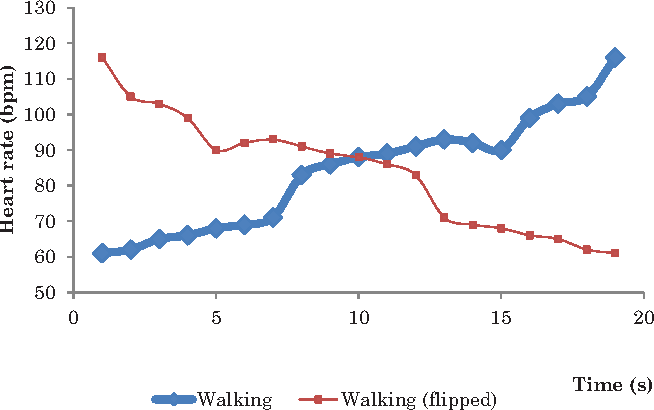
\includegraphics[width=.9\textwidth]{Figures/walking_heart.png}
    \caption{Heart rate signal for walking (bold) and flipped signal (thin) extracted from~\cite{lara2012survey}}
    \label{fig:walking_heart}
\end{figure}

\begin{table}[h]
    \centering
\begin{tabular}{|c|>{\centering}m{8cm}|>{\centering}m{5cm}|}
\hline 
Function & Equation & Parameters\tabularnewline
\hline 
Linear &  \begin{center}
      $F(t)= mt + b$
 \end{center} & \{m, b\}\tabularnewline
Polynomial & \begin{center}
      $F(t)= a_0 + {a_1}t+ ... + a_{n-1}t^{n-1}$ \end{center} & 
      $\{a_0, ..., a_{n-1}\}$ \tabularnewline
Exponential &  \begin{center}
      $F(t)= a{|b|}^t + c$
 \end{center}  &\{a, b, c\}\tabularnewline
Sinusoidal & \begin{center}
      $F(t)= a \times sin(t + b )+ c$
 \end{center} & \{a, b, c\} \tabularnewline
\hline 
\end{tabular}
    \caption{Common functions implemented by structure detectors extracted from~\cite{lara2012survey}}
    \label{tab:structure_features}
\end{table}




The main reason for applying feature extraction on each time window is that it is almost impossible for two given time windows to be exactly identical even if they come from the same subject doing the same activity~\citep{lara2012survey}. On the other words, through that we can filter out relevant information and obtain a quantitative measures of each time window which can further be used to compare with other time windows. In general, feature extraction methods can be categorized into two groups: statistical
and structural~\citep{article}. Regarding the statistical methods, they use quantitative characteristics of the data to extract features. Table~\ref{tab:statistical_features} shows a summery of common statistical features in HAR literature. As for structural methods, however, they consider the interrelationship among data to extract features from signals. In some situations, such features play an extremely significant role in HAR. To illustrate, consider Figure~\ref{fig:walking_heart} which represents the heart rate signal for a person that was walking and the same signal in reverse temporal order. Under such circumstances, statistical features such as time domain and frequency domain features are not discriminative since for these two signals, most of them are equal and we need to use utilize features that take the structure of signals into account. According to~\cite{lara2012survey} and from a mathematical perspective, given a time series $Y(t)$, a structure detector implements a function $f(Y(t)) = \hat{Y}(t)$ such that $\hat{Y}(t)$ approximates $Y(t)$. Table~\ref{tab:structure_features} shows the common functions implemented by structure detectors. In general, choosing the feature extraction method and feature sets are dependent to the nature of signal. For instance, acceleration signals tend to fluctuate and be oscillatory and the features extraction method should be able to handle the high variability of signals.


\subsubsection{Classification}

\begin{table}[h]
    \centering
\begin{tabular}{|c|>{\centering}m{8cm}|>{\centering}m{5cm}|}
\hline 
Classifier & Publications\tabularnewline
\hline 
\hline 
Decision tree &  ~\citep{banos2014window},~\citep{4650398},~\citep{inproceedings},~\citep{Bao2004ActivityRF},~\citep{4650199}\tabularnewline
\hline 
Naive Bayes &~\citep{banos2014window},~\citep{tapia2007real},~\citep{bao2004activity},~\citep{6181018},~\citep{kern2003multi},~\citep{ravi2005activity}\tabularnewline
\hline 
K-nearest neighbors &~\citep{banos2014window},~\citep{4650398},~\citep{inproceedings},~\citep{maurer2006activity},~\citep{ravi2005activity}\tabularnewline
\hline 
Neural Networks &~\citep{8767219},~\citep{al2019deep},~\citep{Wang2018DeepLF}\tabularnewline
\hline 
Support Vector Machines &~\citep{morris2014recofit},~\citep{4620779},~\citep{Wang2018DeepLF},~\citep{4761688},~\citep{Huynh2007ScalableRO},\citep{zhang2011feature}\tabularnewline
\hline 
Markov models &~\citep{Vinh:2011:SCR:2036609.2036624},~\citep{5152756}\tabularnewline
\hline 
Nearest Centroid Classifier &~\citep{huynh2005analyzing}\tabularnewline
\hline 
\end{tabular}
    \caption{Summery of common classifiers in HAR publications }
    \label{tab:classifiers}
\end{table}


Finally, a classifier is trained on the vector of extracted features and corresponding 
labels, and assigns future 
observations to one of the learned activities. Table~\ref{tab:classifiers} summarizes most common classifiers and some work examples of them in the HAR field.  


\subsection{System evaluation}
\label{sub:CVs}
One of the most important step in designing each system is evaluation. The evaluation in HAR has been mostly carried out through k-fold CV. In k-fold CV (Figure~\ref{fig:Shuffle-cv}), the overall data is randomly partitioned in $k$ equal subsets. The model is then trained on $k-1$ subsets, and the remaining one is used for testing~\citep{trevor2009elements}. In this process, the test set can be any part of the dataset meaning that training and test sets may contain the data of same subject and due to that, this method is referred to as subject-dependent CV in literature~\cite{al2019deep}.  
The main assumption of this process is that \emph{samples are Independent and Identically Distributed (i.i.d.)}~\cite{arlot2010survey}, which means that all the data points are sampled independently from the same distribution.  However, samples drawn from a given subject are likely to \emph{not} be independent, for two reasons. First, there is a strong inter-subject variability in the way activities are conducted~\cite{bulling2014tutorial}. This means that the similarity of samples drawn from the same subject is likely to be higher than that of samples drawn from different subjects. Several factors might explain such variability, including sex, gender, age or experience. Second, there is a temporal dependence between activities performed by the same subject: the similarity between samples drawn in a short time interval, for instance in the same training session in case of training activities, will most likely be higher than that of samples drawn further apart in time. This is due to factors such as fatigue and training. Thus, k-fold CV may overestimate the performance of recognizer systems in HAR. Such overestimation is even larger when k-fold CV is used with overlapping sliding windows since the overlap between adjacent windows is another source of dependency between data points. A more formal discussion about the problems of k-fold CV in HAR can be found in~\cite{dehghani2019subject}.   


To address these issues, the training and testing sets should be split by subject. In this method which is known as subject-independent CV~\cite{al2019deep,janidarmian2017comprehensive}, in each iteration the model is trained on all the subjects except one, which is used for testing. In this way, the intra-subject dependencies present in subject-dependent CV are hence removed. It should be noted that, in this case, as is shown in Figure~\ref{fig:Subjective-cv}, the number of folds is lower or equal to the number of subjects in the dataset.    


\begin{figure}[htp]
  \centering
  \subfigure[Subject-dependent CV]
  {\label{fig:Shuffle-cv}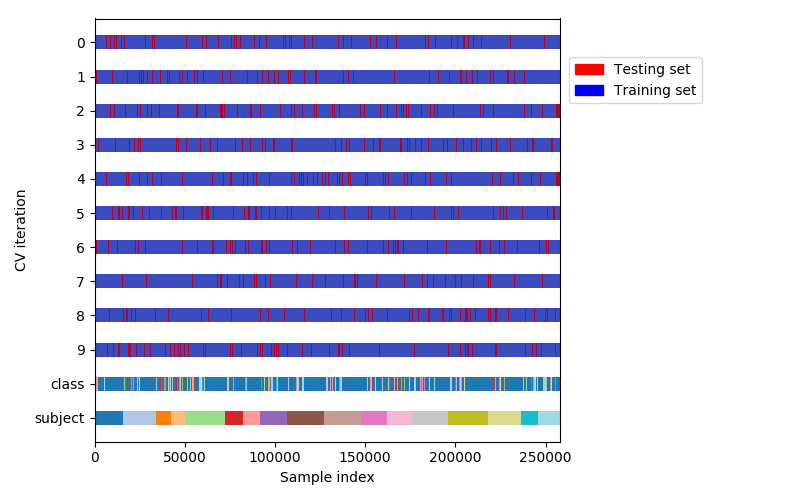
\includegraphics[scale=0.36]{Figures/ShuffleSplit.png}}\quad
  \subfigure[Subject independent CV]
  {\label{fig:Subjective-cv}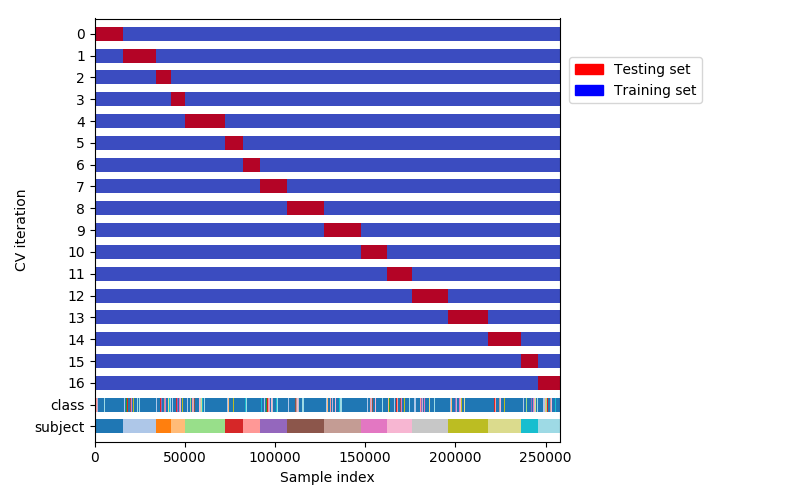
\includegraphics[scale=0.36]{Figures/LeaveOneGroupOut.png}}
   \caption{Different types of CV in HAR}
    \label{fig:CVs}
\end{figure}
\section{Related work}
The sliding window technique is widely employed in HAR, and the literature contains a plethora of examples where both, overlapping (e.g.,~\cite{bao2004activity,tapia2007real,lara2012centinela,morris2014recofit}) and non-overlapping time windows are used (e.g.,~\cite{minnen2007recognizing,reddy2010using,cheng2010active,banos2014window}).
\subsection{Overlapping sliding windows}

The work by Ling Bao and Stephen S. Intille~\cite{bao2004activity} uses overlapping sliding windows to segment signals coming from five biaxial accelerometers placed on 20 subjects (13 males and 7 females) under laboratory and semi-naturalistic conditions while performing 20 daily activities. Subsequently, each window is transformed into a set of features namely mean, energy,  frequency-domain entropy, and correlation of acceleration data. The authors use k-nearest neighbor (KNN), decision tree (DT), and naive bayes (NB) classifiers, and subject-independent cross-validation (CV) and subject-dependent CV for system evaluation. They reach the overall accuracy of 84\% with DT under the subject-independent CV process.

Another example is work by Tapia et al~\cite{tapia2007real} where the authors develop a real-time recognition system to recognize physical activities and in some cases, their intensities. They segment the signal data collected from 21 subjects wearing triaxial wireless accelerometers and a wireless heart rate monitor while performing 30 physical gymnasium activities using overlapping sliding windows. Subsequently, from each window, they extract time domain and frequency domain features and using a DT classifier they recognize activities.with an accuracy of 94.6\% using
subject-dependent CV and 56.3\% using subject-independent CV. 

Lara et al~\cite{lara2012centinela} combine acceleration data with vital signs to improve the performance of HAR systems. They apply ARP on a dataset which was collected from eight subjects (7 males and 1 female) while wearing a BioHarness™ BT chest sensor strap\footnote{\url{http://www.zephyr-technology.com/bioharness-bt.html}}. Using data from a triaxial accelerometer and vital signs, they detect five activities including running, walking, sitting, ascending, or descending. Sensor signals are partitioned into overlapping time windows with three different sizes: 5-seconds, 12-seconds, and 20-seconds sliding at 50\% of their sizes and 90 features were extracted from each time window. NB, DT, Bayesian Network, Multilayer Perceptron, Additive Logistic Regression and classifier ensembles are used to recognize activities. They achieve up to 95.7\% overall accuracy, which was evaluated through subject-dependent CV. Their results also indicate that vital signs are useful to discriminate between certain activities like running and sitting compared to the cases that utilize acceleration data only.


Recofit~\cite{morris2014recofit} is a well-known reference on HAR, which applies ARP on a dataset of accelerometer and gyroscope data collected from 114 participants over 146 sessions. The authors address three major challenges namely (1) 
segmenting exercise from intermittent non-exercise periods, (2) 
recognizing which exercise is being performed, and (3) counting repetitions. Data points are windowed into 5-second overlapping windows sliding at 200 ms and subsequently, each window is transformed into 224 features. Linear support vector 
machines (SVM) are used in the classification stage and evaluated by 
subject-independent CV. Spectacular performance is achieved, with precision and 
recall greater than 95\% to identify exercise periods, recognition 
of up to 99\% for circuits of 4 exercises, and counting  
accurate to $\pm$1 repetition, 93\% of the time.


\subsection{Non-overlapping sliding windows}
Regarding non-overlapping windowing, Minnen et al~\cite{minnen2007recognizing} describes an activity recognition component to recognize soldier activities as a part of the Soldier Assist System (SAS). They apply ARP on the signal of a six three-axis bluetooth accelerometers
positioned on the right thigh sidearm holster to recognize 14 soldier activities. The sensor signals are partitioned by 3-second non-overlapping sliding windows and then each window is transformed into 378 features. A boosting ensemble classifier is used to select the most important features and also recognize the activities. Their recognition system achieves 78.7\% for continuous event recognition (considering null activity)
and 70.3\% frame level accuracy. These values increase to
90.3\% and 90.3\% ,respectively when considering only the
modeled activities. In their study, they use subject-independent CV to evaluate their system. 

Another example is the work by REDDY et al~\cite{reddy2010using}, where the authors create a transportation mode recognition system using a mobile phone to identify whether
an individual is stationary, walking, running, biking, or in motorized transport. The dataset used in their study contains accelerometer measurements, GPS, WiFi, and GSM signals of sixteen individuals (eight male and eight female) while six phones attached to their bodies simultaneously and were in one of the five transportation modes for fifteen minutes. The signals are windowed into 1-second non-overlapping sliding windows and each window is transformed into a set of features such as magnitude of the force vector, mean, variance, energy, etc. They use several classifiers namely DT, NB, KNN, SVM, Hidden Markov
Model and a two-stage classifier involving DT combined with discrete
Hidden Markov Model. They achieve an accuracy level of 93.6\% with the two-stage classifier, which was evaluated by subject-dependent CV.

Cheng et al~\cite{cheng2010active} implement an on-body capacitive sensing approach to recognize activities such as chewing, swallowing, speaking, sighing (taking a deep breath), as well as
different head motions and positions. They use a dataset that contains the 4.3 hours-electrode collar data which was collected from three subjects (one female, two males; aged between 25 and 45 years) while performing a set of head movements, swallow water from a cup, chew and swallow bread pieces and speak. Each signal is partitioned into 1.5-second non-overlapping sliding windows and each window then is transformed into time domain features such as signal mean, variance, maximum, etc. They use a linear discriminant
classifier to identify various activities and evaluate the system through subject-dependent CV and report the accuracy rate for the combination of activities.  

Another example is the work by Banos et al~\cite{banos2014window}, where the authors present an extensive study to distinguish the windowing procedure, its impacts on the recognition system. They apply ARP on the accelerometer data of a benchmark dataset collected from 17 subjects of different profiles performing 33 fitness activities in an out-of-lab environment. Sensor signals are windowed into non-overlapping windows with a substantial set of window sizes ranging from 0.25 to 7 seconds in steps of 0.25-seconds. Each window is then transformed into three different feature sets (FS) namely FS1 (mean only), FS2 (mean and standard deviation) and FS3 (mean, standard deviation, maximum, minimum and mean crossing rate). They use DT, KNN (K=3), NB and Nearest Centroid Classifier (NCC) as the classifiers and subject-dependent CV for system evaluation. From this study, they prove that the interval 1–2 second is the best trade-off between recognition speed and performance. Besides, they provide a set of guidelines for system definition and configuration based on the particular application requirements and target activities.